\chapter{Efficient model utilization}



\section{Low-rank adaptation} \label{sec:lora}

\begin{description}
    \item[Low-rank adaptation (LoRA)] \marginnote{Low-rank adaptation (LoRA)}
        Method to update weights by learning an offset that uses fewer parameters.

        Consider a weight matrix $\matr{W} \in \mathbb{R}^{d \times k}$, LoRA decomposes the update into two learnable matrices $\matr{A} \in \mathbb{R}^{d \times r}$ and $\matr{B} \in \mathbb{R}^{r \times k}$ (with $r \ll d, k$). Weights update is performed as:
        \[ \matr{W}_{\text{fine-tuned}} = \matr{W}_{\text{pre-trained}} + \matr{AB} \]

        \begin{figure}[H]
            \centering
            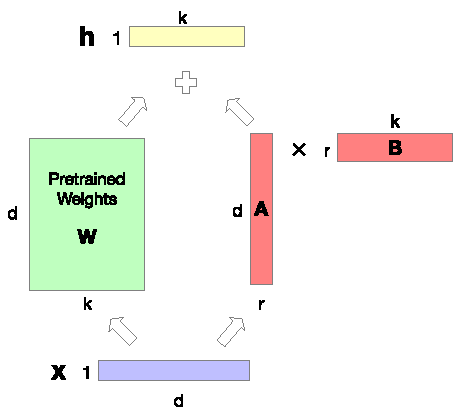
\includegraphics[width=0.4\linewidth]{./img/_lora.pdf}
        \end{figure}
\end{description}



\section{Model compression}


\subsection{Parameters compression}

\begin{description}
    \item[Parameter sharing] \marginnote{Parameter sharing}
        Use the same parameters between layers.

    \item[Pruning] \marginnote{Pruning}
        Remove weights with small impact on the loss.

        \begin{remark}
            Dropping some weights produce sparse matrices that are unoptimized for parallel hardware. Therefore, this approach does not always improve efficiency.
        \end{remark}

    \item[Quantization] \marginnote{Quantization}
        Store and perform operations with lower precision floating-points (e.g., FP32 to FP4).
\end{description}


\subsection{Training compression}

\begin{description}
    \item[Mixture of experts] \marginnote{Mixture of experts}
        Specialize smaller models on subset of data and train a router to forward the input to the correct expert.

        \begin{remark}
            This approach can be easily deployed on distributed systems.
        \end{remark}

    \item[Knowledge distillation] \marginnote{Knowledge distillation}
        Train a student model to emulate the teacher's hidden states. In a general setting, the output distribution of the teacher is used to create the student. Two losses are used:
        \begin{descriptionlist}
            \item[Distillation loss] 
                Matches the output distribution of the student to the one of the teacher. A softmax with higher temperature is usually used so that training contribution does not only come from the highest probability.

            \item[Student loss] 
                Matches the output distribution of the student with the ground-truth (i.e., same loss of the training task).
        \end{descriptionlist}

        \begin{figure}[H]
            \centering
            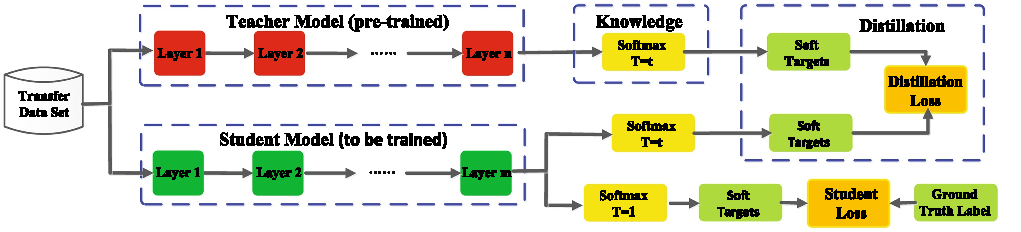
\includegraphics[width=0.8\linewidth]{./img/_distillation.pdf}
        \end{figure}

    \item[Vocabulary transfer] \marginnote{Vocabulary transfer}
        Use a domain-specific tokenizer to reduce the number of tokens to represent complex/domain-specific words and reduce the size of the embedding matrix.

        \begin{description}
            \item[Fast vocabulary transfer (FVT)] \marginnote{Fast vocabulary transfer (FVT)}
                Given:
                \begin{itemize}
                    \item A starting embedding model with tokenizer $\mathcal{T}_\text{s}$, vocabulary $V_\text{s}$, and embedding matrix $\matr{E}_\text{s}$,
                    \item A new tokenizer $\mathcal{T}_\text{dom}$ trained on a domain-specific corpus,
                \end{itemize}
                The embedding matrix $\matr{E}_\text{dom}$ for the vocabulary $V_\text{dom}$ of $\mathcal{T}_\text{dom}$ is built as follows:
                \[ 
                    \forall t_i \in V_\text{dom}: \matr{E}_\text{dom}(t_i) = \frac{1}{|\mathcal{T}_\text{s}(t_i)|} \sum_{t_j \in \mathcal{T}_\text{s}(t_i)}\matr{E}_\text{s}(t_j)
                \]
                In other words, each token in $V_\text{dom}$ is encoded as the average of embeddings of the tokens that compose it in the starting embedding model (if the token appear in both vocabularies, the embedding is the same).
        \end{description}

\end{description}